\documentclass[twoside,10pt]{article}
\usepackage{/Users/bradenhoagland/latex/styles/toggles}
%\toggletrue{sectionbreaks}
%\toggletrue{sectionheaders}
\newcommand{\docTitle}{HW 1}
\usepackage{/Users/bradenhoagland/latex/styles/common}
\importStyles{modern}{rainbow}{boxy}

%\renewcommand{\theenumi}{\alph{enumi}}

\begin{document}
%\tableofcontents

% ------------------------------
% 1.1
% ------------------------------
\begin{exer}[1.1]
Distance between earth and star.
\end{exer}

Assuming Euclidean geometry, the angles in the below diagram sum to $180\degree$. Thus the unmarked angle is $0.1\degree$. Then by the law of sines,
\[
	\frac{a}{\sin(100.8\degree)} = \frac{b}{\sin(79.1\degree)} = \frac{186}{\sin(0.1\degree)} .
\] Solving yields $a \approx 104682$ and $b \approx 104647$. Everything here was done in terms of millions of miles, so the distance between the star and the earth is approximately 100,000,000,000 miles.

\begin{center}
	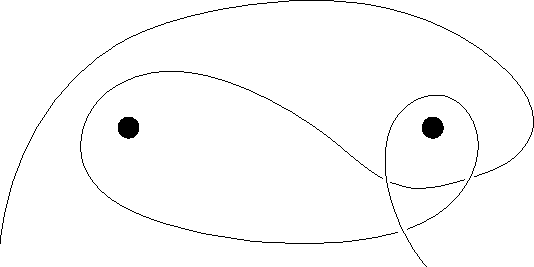
\includegraphics[scale=0.7]{fig/1}
\end{center}

\newpage

% ------------------------------
% 1.7
% ------------------------------
\begin{exer}[1.7]
	Pappus' Variation on the Pythagorean Theorem.
\end{exer}

\begin{center}
        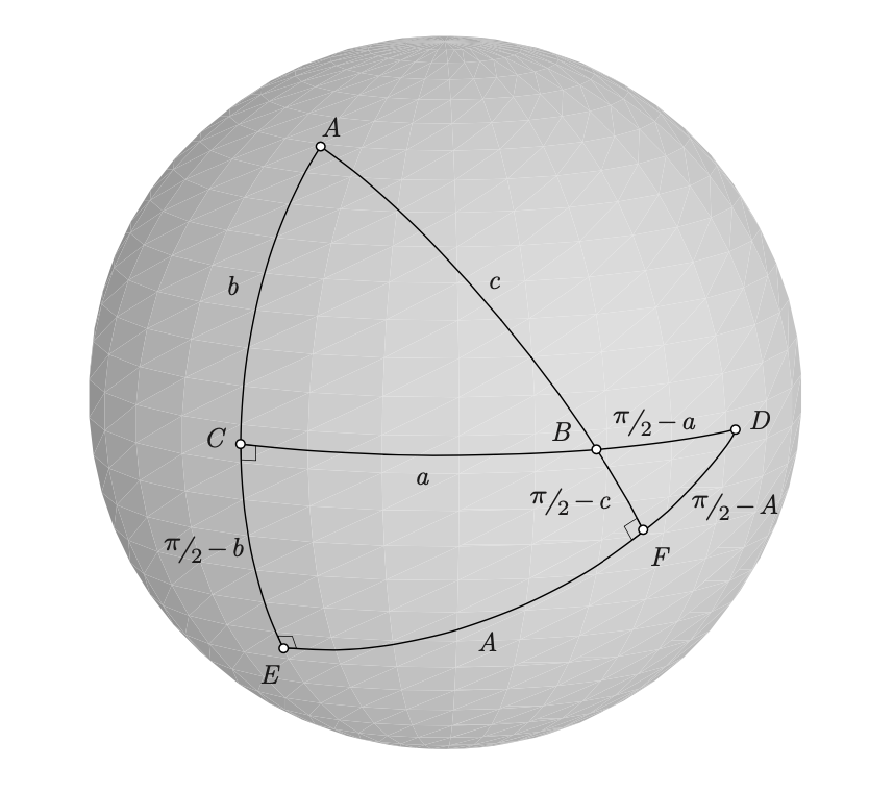
\includegraphics[scale=0.7]{fig/21}
\end{center}

Since a sheared image of a parallelogram has the same base and height, it has the same area, and thus any shear preserves area. Thus we can shear both $\mathcal{A}$ and $\mathcal{B}$ onto the bottom-left copy of $\mathbf{v}$ to get the following image.

\begin{center}
        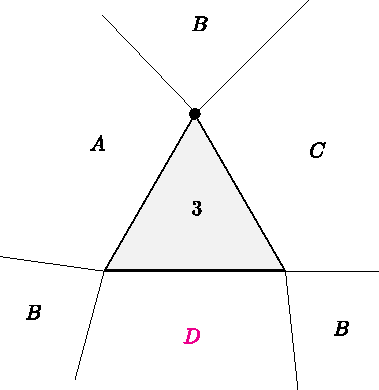
\includegraphics[scale=0.7]{fig/22}
\end{center}

Now shear $\mathcal{A}'$ onto $\mathcal{C}_1$ and shear $\mathcal{B}'$ onto $\mathcal{C}_{2}$. Since we have completely filled $\mathcal{C}$ with parallelograms of the same area as $\mathcal{A}$ and $\mathcal{B}$, we have
\[
	\text{Area}(\mathcal{A}) + \text{Area}(\mathcal{B}) = \text{Area}(\mathcal{C}).
\] 

\newpage

% ------------------------------
% 1.15
% ------------------------------
\begin{exer}[1.15]
	Isometry with 2 fixed points is either the identity or a reflection.
\end{exer}

Suppose $f$ is an isometry with fixed points $P,Q$.

\textbf{All points in the line through $P$ and $Q$ are also fixed points:} Let $R$ be on the line $\ell$ through $P$ and $Q$. Draw two circles: one at $P$ with radius $|PR|$ and the second at $Q$ with radius $|QR|$. By lemma 1.3.2, since $R$ is on $\ell$, these two circles intersect at only one point ($R$ itself). But then since $f$ preserves distances, this singular point is the only possible destination for $R$, i.e. $f(R) = R$.

\textbf{Either identity or reflection:} Now we show that $f$ must be either the identity map or a reflection through $\ell$. Let $R$ be any point not on $\ell$. Again we draw two circles, one at $P$ with radius $|PR|$ and the second at $Q$ with radius $|QR|$. Since $R$ is not on $\ell$, these circles intersect at two points (one of which must be $R$). Thus $f$ can either map $R$ to itself or to that second point $R'$.

Now fix a point $S \neq R$ not on $\ell$. This point $S$ has a similar situation, in that it can either be mapped to itself or to one other point $S'$. We claim that $R$ is a fixed point if and only if $S$ is a fixed point.

\begin{itemize}
	\item Suppose $R$ is a fixed point. If $S$ is mapped to $S'$, then its distance to $R$ is different, contradicting that $f$ is an isometry.

	\item Suppose $S$ is not a fixed point, then by a similar argument, $f$ must map $R$ to $R'$ in order to preserve distance.
\end{itemize}

Thus in one case, all of $\mathbb{R}^2-\ell$ is mapped to itself, i.e. $f=\id_{}$. In the other case, no point in $\mathbb{R}^2-\ell$ is fixed, i.e. $f$ is a reflection.

\newpage

% ------------------------------
% 1.17
% ------------------------------
\begin{exer}[1.17]
	If $\ell_1\neq \ell$ is sent to itself under a reflection through $\ell$, then $\ell_1$ and $\ell$ intersect at right angles.
\end{exer}

Suppose $f$ is the reflection through $\ell$, and fix an angle $\theta$ at the intersection of $\ell$ and $\ell_1$. Since isometries preserve angles, $f(\theta)$, one of the adjacent angles of $\theta$, is congruent to $\theta$. Thus $\ell$ and $\ell_1$ intersect at right angles.

\begin{center}
        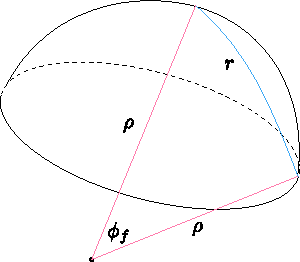
\includegraphics[scale=0.7]{fig/3}
\end{center}

\newpage

% ------------------------------
% 1.22
% ------------------------------
\begin{exer}[1.22]
Show that the interior angles in a quadrilateral sum to $360\degree$. Generalize this to $n$-gons.
\end{exer}

We claim that for any $n$-gon, the sum of the interior angles is
\[
	(n-2) \cdot 180\degree.
\] We begin with the simple case of a quadrilateral.

Suppose we have a quadrilateral $ABCD$, then we can decompose this into two triangles $ABD$ and $BCD$. Since the interior angles of a triangle sum to $180\degree$, the interior angles of $ABCD$ must sum to $2 \cdot 180\degree = 360\degree$. Note that this satisfies the original claim.

We now extend this result through induction. Suppose the hypothesis holds for all $n$-gons, then we must show it holds for all $(n+1)$-gons. Let $X_1\cdots X_{n+1}$ is an $(n+1)$-gon with points labeled clockwise, then we can decompose it into the $n$-gon $X_1\cdots X_{n}$ and the triangle $X_{n}X_{n+1}X_1$. By our inductive hypothesis and the fact that the interior angles of a triangles sum to $180\degree$, the sum of our $(n+1)$-gon's interior angles is
\[
	(n-2) \cdot 180\degree + 180\degree = \left( (n+1)-2 \right) \cdot 180\degree.
\] Thus all $n$-gons satisfy the original claim.

\newpage

% ------------------------------
% 1.23
% ------------------------------
\begin{exer}[1.23]
What is the sum of the exterior angles of an $n$-gon?
\end{exer}

Let $E_i$ denote the $i$-th exterior angle of our $n$-gon. By definition, it is adjacent to the $i$-th interior angle $I_{i}$. By the previous exercise, the sum of all the $E_{i}$ is
\[
	\sum_{i=1}^{n} E_{i} = \sum_{i=1}^{n} (180\degree - I_{i}) = n \cdot 180\degree - (n-2)\cdot 180\degree = 360\degree.
\] 
Thus the sum of the exterior angles of all $n$-gons is $360\degree$.

\newpage

% ------------------------------
% 1.28
% ------------------------------
\begin{exer}[1.28]
	If $ABC$ is a right inscribed angle, then $AC$ is a diameter.
\end{exer}

Suppose $ABC$ is a right inscribed angle in a circle of origin $O$ and radius $r$ as pictured below. Then by the Star Trek Lemma, the angle $AOC$ is $2 \cdot 90\degree = 180\degree$. Then $AC$ is a straight line through the center of the circle of length $2r$, i.e. a diameter.

\begin{center}
        \includegraphics[scale=0.7]{fig/4}
\end{center}

\newpage

\end{document}
